\documentclass[a4paper,12pt]{scrartcl}
\usepackage{tikz}
\usepackage{amsmath}
\usetikzlibrary{shapes.misc}
%\usepackage{showframe}

\begin{document}
\title{Probleme d'Equation de Simulation d'Epidemie - Equation Differentielle par Integration en Separant les Variables}
\author{Elliot Jullier}
\date{\today}
\maketitle

\pagenumbering{roman}
\tableofcontents
\newpage
\pagenumbering{arabic}

\section{Modèle SIR}
\subsection{Le Principe}

\begin{center}
    \emph{"Tout les modèles sont faux... mais il y en a qui sont utiles" - George Box}
\end{center}
Cette citation exemplifie la nécéssité des modèles pour avoir une approximation plus 
ou moins fidele à la realite. Il existe plusieurs modèles possibles pour cette modélisation mathématique, 
mais dans ce papier nous allons seulement commencer à étudier les plus simples. Notamment le modèle dit SIR.
\\ \\
Dans ce modèle, on départage une population ayant $N$ individus, on considere dans ce modèle que la population
reste constante, alternativement, on peut dire que le taux de mortalité reste très faible comparé à la population totale. Il y a trois classes:
\begin{enumerate}
    \item 'S': La population qui est susceptible à se faire infecté.
    \item 'I': La population qui est infecté et contagieuse -  le vecteur de transmission d'epidemie en question.
    \item 'R': La population résistante à l'infection et ne peuvent plus l'être (dans ce modèle). Ils ont été contagieux, mais ne le sont plus. 
\end{enumerate}

\subsection{Le Schema}

\vspace{10mm}

\begin{center}

    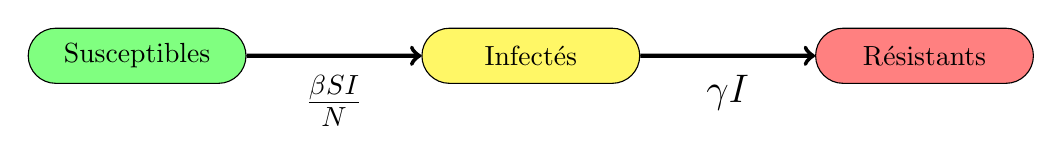
\begin{tikzpicture}
        \draw (0,0) node(S) [draw, 
            fill=white!50!green,
            rounded rectangle, 
            minimum width = 3cm, 
            minimum height = 0.7cm] 
        {Susceptibles};
        \draw (5,0) node(I) [draw, 
            fill=white!40!yellow,
            rounded rectangle, 
            minimum width = 3cm, 
            minimum height = 0.7cm] 
        {Infectés};
        \draw (10,0) node(R) [draw, 
            fill=white!50!red,
            rounded rectangle, 
            minimum width = 3cm, 
            minimum height = 0.7cm] 
        {Résistants};
        \draw[ultra thick, ->] (S) -- (I);
        \draw[ultra thick, ->] (I) -- (R);
        \draw (S) -- (I) node[midway, label=below:\Large $\frac{\beta SI}{N}$ \normalsize] {};
        \draw (I) -- (R) node[midway, label=below:\Large $\-\gamma I$ \normalsize] {};
    \end{tikzpicture}

    \emph{Figure 1 - Etats et Transition dans un Modèle SIR}
    \label{Figure 1}

\end{center}

\subsection{Explication des Taux de Transition}
\begin{itemize}
    \item[-] $\frac{dS}{dt}$: Premièrement, on prends $\frac{S}{N}$ comme la fraction de la population totale qui est 
        susceptible à être infecté, de plus on prends $\frac{I}{N}$ la fraction de la population déjà infecté. 
        Logiquement, le nombre de nouvelles personnes infectées depends du nombre de personnes susceptibles de l'être
        et du nombre de personnes deja infectées. Donc on peut en deduire que la fraction des contactes entre un individu 
        susceptible et un individu infecté qui résulte en la transmission de l'infection est alors de: 
        $\frac{S}{N} \times  \frac{I}{N} = \frac{SI}{N^2}$ \\
        Deuxièment, on note $\beta$ le nombre moyen de contactes par personne infecté par unité de temps.\\
        Finalement, on peut donc déduire que pour chaque individu infecté, il y a un individu en moins qui est
        susceptible. Donc $\frac{d\frac{S}{N}}{dt} = \frac{-\beta SI}{N^2}$ or $N$ est constant donc $\frac{d\frac{S}{N}}{dt}=\frac{1}{N}\times \frac{dS}{dt}$ 
        \\ Donc on a: \[ \boxed{\frac{dS}{dt} = \frac{-\beta SI}{N}}\]
    \item[-] $\frac{dI}{dt}$: Il tient de la \emph{Figure 1} dans la Section \ref{Figure 1} (p. \pageref{Figure 1}) que toute 
        population qui n'est plus susceptible devient alors infecté. De plus, il faut prendre en compte qu'il y a des personnes qui 
        'partent' de la classe 'Infectés' et deviennent alors 'Resistants'. 
        \\ Donc il tient que: \[ \boxed{ \frac{dI}{dt} = \frac{\beta SI}{N}-\gamma I}\] 
    \item[-] $\frac{dR}{dt}$: De nouveau, d'après la \emph{Figure 1} on sait que personne ne quitte la population 
        'Résistante' et que seuls les infectés peuvent devenir resistants. Or le taux de ceux qui sorte de la categorie 
        'Infecté' est de $- \gamma I$ \\ donc: \[ \boxed{\frac{dR}{dt} = \gamma I} \]
    \item[-] De plus, nous avons postulé que, dans ce modèle, la population totale reste fixe et comme les classes $S$, $I$ et $R$ forment
        l'integralite de $N$ alors, on a: \\
        \[\frac{dS}{dt}+\frac{dI}{dt}+\frac{dR}{dt} = \frac{dN}{dt} \Leftrightarrow \frac{dN}{dt}=\frac{-\beta SI}{N} + \frac{\beta SI}{N}-\gamma I + \gamma I = 0\] 
        \\ En effet une population constante engendre que le taux de variation de la population est 0. 
\end{itemize}


\section{Modelisation du Modèle SIR en Fonction du Temps}

\end{document}